\documentclass[a4paper, twoside]{report}

%% Language and font encodings
\usepackage[english]{babel}
\usepackage[utf8]{inputenc}
\usepackage[T1]{fontenc}

%% Sets page size and margins
\usepackage[a4paper,top=3cm,bottom=2cm,left=3cm,right=3cm,marginparwidth=1.75cm]{geometry}

%% Useful packages
\usepackage{amsmath}
\usepackage{CJKutf8}
\usepackage{xspace}
\usepackage{graphicx}
\usepackage{array, booktabs}
\usepackage{listings}
\usepackage[dvipsnames]{xcolor}
\usepackage{textcomp}
\usepackage{wrapfig}
\usepackage[colorinlistoftodos]{todonotes}
\usepackage[colorlinks=true, allcolors=blue]{hyperref}

% Separation logic style sheet
\usepackage{sl}
\usepackage{gillian}

\setlength{\parindent}{0em}
\setlength{\parskip}{1em}

% Formatting for code listings
\lstdefinestyle{code}{
    commentstyle=\color{ForestGreen},
    keywordstyle=\color{Blue},
    stringstyle=\color{OliveGreen},
    basicstyle=\ttfamily\small,
    showstringspaces=false,
    upquote=true,
    numbers=left,
    numberstyle=\scriptsize\color{Gray},
    frame=lines
}
\lstdefinestyle{code-inline}{
    commentstyle=\color{ForestGreen},
    keywordstyle=\color{Blue},
    stringstyle=\color{OliveGreen},
    basicstyle=\ttfamily\small,
    showstringspaces=false,
    upquote=true,
    numberstyle=\scriptsize\color{Gray},
    xleftmargin=\parindent
}
\lstdefinestyle{terminal}{
    basicstyle=\ttfamily\footnotesize,
    showstringspaces=false,
    upquote=true,
    frame=lines
}
\lstdefinestyle{terminal-inline}{
    basicstyle=\ttfamily\small,
    showstringspaces=false,
    language=bash,
    upquote=true,
    xleftmargin=\parindent,
}

\title{Interim Report - Gillian Debugging}
\author{Nat Karmios}

\begin{document}

% Text in \autoref references
\def\chapterautorefname{\normalcolor{Chapter}\color{blue}}
\def\sectionautorefname{\normalcolor{\S}\kern-0.7ex\color{blue}}
\def\subsectionautorefname{\normalcolor{\S}\kern-0.7ex\color{blue}}
\def\figureautorefname{\normalcolor{Figure}\color{blue}}
\def\lstnumberautorefname{\normalcolor{line}\color{blue}}

\begin{titlepage}

\newcommand{\HRule}{\rule{\linewidth}{0.5mm}} % Defines a new command for the horizontal lines, change thickness here

%----------------------------------------------------------------------------------------
%	LOGO SECTION
%----------------------------------------------------------------------------------------


\includegraphics[width=8cm]{title/logo.eps}\\[1cm] % Include a department/university logo - this will require the graphicx package

%----------------------------------------------------------------------------------------

\center % Center everything on the page

%----------------------------------------------------------------------------------------
%	HEADING SECTIONS
%----------------------------------------------------------------------------------------

\textsc{\LARGE MEng Individual Project}\\[1.5cm] % Name of your university/college
\textsc{\Large Imperial College London}\\[0.5cm] % Major heading such as course name
\textsc{\large Department of Computing}\\[0.5cm] % Minor heading such as course title

%----------------------------------------------------------------------------------------
%	TITLE SECTION
%----------------------------------------------------------------------------------------
\makeatletter
\HRule \\[0.4cm]
{ \huge \bfseries \@title}\\[0.4cm] % Title of your document
\todo{Change project title!}
\HRule \\[1.5cm]

%----------------------------------------------------------------------------------------
%	AUTHOR SECTION
%----------------------------------------------------------------------------------------

\begin{minipage}{0.4\textwidth}
\begin{flushleft} \large
\emph{Author:}\\
\@author % Your name
\end{flushleft}
\end{minipage}
~
\begin{minipage}{0.4\textwidth}
\begin{flushright} \large
\emph{Supervisor:} \\
Prof. Philippa Gardner \\[1.2em] % Supervisor's Name
\emph{Second Marker:} \\
Dr. Robert Chatley % second marker's name
\end{flushright}
\end{minipage}\\[2cm]
\makeatother

% If you don't want a supervisor, uncomment the two lines below and remove the section above
%\Large \emph{Author:}\\
%John \textsc{Smith}\\[3cm] % Your name

%----------------------------------------------------------------------------------------
%	DATE SECTION
%----------------------------------------------------------------------------------------

{\large \today}\\[2cm] % Date, change the \today to a set date if you want to be precise

\vfill % Fill the rest of the page with whitespace

\end{titlepage}


\tableofcontents

%!TEX root = ../main.tex

\chapter{Introduction}\label{sec:intro}

% Setting the question - what is the goal? Give broad strokes on the setting -
% analysis tools, bi- vs verification, accessibility for code developers
As programs become larger and more complex, how do we guarantee the correctness
of code? Symbolic analysis tools are becoming increasingly promising as research
and development continues. These generally come in the form of {\bf a)}
automated testing via bi-abduction, where code is submitted as-is for symbolic
executed, with potential errors (such as divide-by-zero and null dereferences)
reported as a result, and {\bf b)} full program verification, where code is
annotated with logical conditions (pre-conditions, post-conditions, loop
invariants, etc.); 

% State of the art; VeriFast, but it only does this; previous MEng,
% but they only do this; Julian Dolby (ask Sacha)?

% What I've done, and how; either break this down, or talk about most interesting

% Ending; a bigger goal; undergrads, then code developers 

% It is an inevitable truth that the complexity of programs and their codebase
% will continuously grow. As this happens, how can one guarantee code does what
% it needs to?

% Symbolic analysis tools are becoming an increasingly promising choice as
% research and development into a plethora of projects continue (some of which
% are discussed in \autoref{sec:background:sl-and-tools}). The benefit of using
% symbolic methods over ones dependent on concrete execution (i.e.\ unit tests) is
% that they cover all possible states of execution without needing to specify each
% scenario by hand.

% Enter
% Gillian~\cite{gillian-santos,gillian-part1,gillian-part2,gillian-techrep}.
% Created by Imperial College London's Verified Software group, it
% is a platform for the development of symbolic analysis tools. Compared to
% related projects, Gillian has two advantages.
% Firstly, it is \textit{parametric} on the target language's (TL) memory model;
% if provided with a compiler from a TL to GIL (a simple, Gillian-specific
% GOTO language) and an implementation of the TL's memory model (in OCaml),
% then Gillian can do all the heavy lifting and perform symbolic analysis on programs written in that
% TL in various ways~\cite{gillian-part1}. This brings to front Gillian's second advantage; it supports three methods of symbolic
% analysis:
% \begin{itemize}
%   \item \emph{Whole program symbolic testing}, in which developers write a
%   number of unit tests with symbolic inputs and outputs, as well as constraints
%   on the outputs in first-order logic. Gillian then attempts to find a symbolic
%   state that invalidates those assertions.

%   \item \emph{Full verification}: developers annotate functions with pre- and
%   post-conditions, loop invariants, and proof tactics, in the style of
%   separation logic; Gillian then symbolically executes the functions with
%   pre-conditions intact to see if the post-conditions hold.

%   \item \emph{Automatic compositional testing}. Similarly to Facebook's
%   Infer~\cite{infer, infer-site}, developers submit a program without any
%   pre-conditions, post-conditions, or any other logical annotations, and,
%   through bi-abduction\cite{bi-abduction}, Gillian will respond with
%   separation logic-style specifications for that programs behaviour, up
%   to a specified bound.
% \end{itemize}

% Whilst symbolic analysis tools have clear benefits when proving program
% correctness, the adoption of symbolic methods in industry remains limited; a
% strong factor to this end is the lack of IDE support for
% developers~\cite{magpiebridge}.
% In addition, in the specific case of Gillian, upon failure of any analyses, a
% user has to sift through a multi-megabyte log file to find the offending piece
% of GIL code; deducing both the cause of the error and the location of the
% problems in the original TL code would take an unreasonable amount of work and
% understanding~\cite{gillian-debugging-2021}.

% To assuage these issues, significant work has gone into developing a debugger
% for Gillian's verification process, as well as improving its error reporting.
% This undertaking, in its state before this project, made use of the DAP (debug adapter
% protocol) with the goal of providing a debugger than can be dropped into any IDE that supports
% it, with little-to-no integration required with any specific IDE.\@ Whilst this
% debugger did improve the user experience of Gillian, the DAP only
% provided a limited amount of functionality, primarily designed for debugging
% concrete execution.\@ The decision had been taken to work within these
% limitations, producing a debugger that can successfully step over, into and out
% of (GIL, WISL, or JavaScript) code. An unfortunate consequence of this decision
% is that a number of much desired features could not be provided, such as `the
% ability to choose which branch to go down on a conditional statement' and
% `better visualisations of the current execution tree'
% ~\cite[p.~49]{gillian-debugging-2021}.

% The decision to use the DAP instead of a custom solution was made, quite
% reasonably so, due to `the short timeframe of a Master's project'. Standing on
% the shoulders of previous work to this end, this project takes Gillian's
% debugging tools beyond the limitations of the DAP, and provides an experience
% befitting real users, rather than experimental scenarios. In particular, the
% contributions of this project are as follows:
% \begin{itemize}
%   \item completely restructuring Gillian's database logging to more strongly
%         resemble an intuitive understanding of symbolic execution and
%         unification, without affecting the existing file logging mechanism
%         (\autoref{sec:log-structure});
%   \item overhauling Gillian's symbolic interpreter to support executing commands
%         at any branch path, rather than executing each branch one after the
%         other in a depth-first fashion, while still supporting the original
%         behaviour (\autoref{sec:interpreter-branching});
%   \item creating and populating navigable data structures to aid in the
%         traversal of both symbolic execution and the unification process
%         (\autoref{sec:navigating-symex}, \autoref{sec:debug-unify});
%   \item extending the existing set of Debug Adapter Protocol commands to allow
%         for an expansive set of debugging capabilities not limited by rigid
%         adherence to the DAP (\autoref{sec:dap-custom}); and
%   \item creating a visual, feature-rich debugging UI, allowing selective
%         step-by-step symbolic execution and a deep inspection of the unification
%         process (\autoref{sec:debug-interface}).
% \end{itemize}

%!TEX root = ../main.tex

\chapter{Background}
\label{sec:background}

\section{Separation Logic}

Proposed in 1969, Tony Hoare's \textit{Hoare Logic} provided a standardised
means of reasoning about programs and their correctness~\cite{hoare}. The key
principle of this logic is the Hoare Triple, denoting that if a certain
pre-condition $P$ holds, and code command $C$ is run (and terminates without
failing), then the post-condition $Q$ is guaranteed to hold. This is presented
in the form of a \textit{Hoare triple}:
$$
  \triple{P}{C}{Q}
$$

Whilst this is a strong foundation for reasoning about programs, anything more
than the simplest of functions become hugely cumbersome to work with,
particularly concerning operations on heap-allocated memory. In 2001, Peter
O'Hearn and John Reynolds proposed \textit{Separation Logic} as the solution to
this~\cite{separation-logic}. Separation Logic reasons about
\textit{heap fragments} (sometimes called \textit{heaplets}), which represent
sections of a theoretical computer's heap; it also provides three core features
in addition to the standard Hoare Logic:

\begin{figure}[!b]
  \centering
  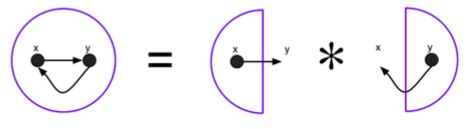
\includegraphics[width=200px]{img/separating-conjunction.jpg}
  \caption{
    A visualisation of the separating conjunction.
    From~\cite{infer-sl}.
  }
  \label{fig:separating-conjunction}
\end{figure}

\begin{itemize}
  \item The \textit{heap cell assertion}, $\cell{x}{y}$, denotes that a heap
  fragment composes of a single cell at address $x$ with value $y$.

  \item The \textit{separating conjunction}, $P \lstar Q$, states that the heap
  fragment can be split into two disjoint (potentially empty) sub-fragments,
  one of which satisfies $P$, and the other satisfies~$Q$.

  \item The \textit{Frame Rule} - a fundamental rule that allows derivations to
  temporarily ``forget'' any unneeded logic either not concerning
  heap-allocated memory, or concerning heap-allocated memory that isn't mutated
  by the command(s) currently being considered. Intuitively, this states that
  any programs that can execute on a state $P$ can also execute on a larger
  state, $P \lstar R$. The Frame Rule is as follows:

  $$
    \inferrule[Frame]{
      \triple{P}{C}{Q} \quad \mathtt{mod}(C) \cap \mathtt{fv}(R) =
      \emptyset}{\triple{P \lstar R}{C}{Q \lstar R}
    }
  $$
\end{itemize}

\polish{PM: Sentence about how SL has served as a basis for various tools and success stories, from academia to industry---SmallFoot, Abductor, Infer, Verifast, Gillian---this links well with the upcoming tools. Not sure about VeriFast.}

\section{OCaml}

Created in 1996, \textit{OCaml}~\cite{ocaml} is `an industrial-strength
programming language supporting functional, imperative and object-oriented
styles'. Specifically, OCaml provides the ability to make use of functional,
imperative, and object-oriented styles. This, combined with its powerful type
system, makes it a good fit for symbolic analysis tools. Many of Gillian's
contemporaries, including Infer~\cite{infer}, VeriFast~\cite{verifast-paper,
verifast-repo}, and Frama-C~\cite{frama-c}, are also written in OCaml.

OCaml's most popular build system is \textit{Dune}~\cite{dune} - it allows the
easy compilation of multi-file OCaml programs and libraries, including
dependencies from \textit{OPAM}~\cite{opam}, OCaml's designated public library
repository. Despite Dune's popularity, it is a fairly bare-bones system, quickly
growing cumbersome when developing larger projects and, in particular,
switching development between projects; Dune requires that OPAM dependencies
are installed system-wide, which can lead to inconsistent builds and version
conflicts. The answer to these concerns is \textit{esy}~\cite{esy}, a package
management system for OCaml and Reason styled after \textit{npm}~\cite{npm}.
Esy provides `provides a fast and powerful workflow for local development of
opam packages without requiring ``switches''', meaning dependencies are isolated
between projects. Esy also provides a number of convenience features, such as
defining custom commands that run within the OCaml project's environment, as
well as supporting non-OPAM dependencies, e.g. OCaml sources from GitHub
repositories (optionally at a specific commit).


%% Described in Intro
%\section{Gillian}
%\section{Debugging - previous work}

\section{Related Tools}
\label{sec:background:related-work}

We consider several closely related tools, namely Infer, Verifast, and Frama-C, and outline their error-reporting and debugging capabilities.

\myparagraph{Infer}
Facebook's \textit{Infer}~\cite{infer, infer-site} is a static analysis tool
for Java and C/C++/Objective-C, designed to use bi-abduction to provide users
with a list of potential bugs, crashes, and sources of poor performance.
Similarly to Gillian, Infer is written in OCaml, and works by compiling source
code to an intermediate representation. In contrast, Infer wholly focuses on
automated compositional testing, and refines this process to a state in which
it can easily be used in industry, whilst also including more general analysis
for concerns such as security and concurrency; it sacrifices depth of analysis
to result in a lightweight tool that gives developer-friendly feedback.

Infer doesn't require the a full program in order to perform analysis, as it
only needs to construct Hoare triples for one function at a time. This,
combined with its ability to reuse existing results from unchanged functions to
only consider modified code, makes for a fast and hugely scalable static
analysis tool, used as part of Facebook's code quality pipeline for all
modifications to the Android and iOS apps for Facebook, Facebook Messenger,
Instagram, and others services~\cite{infer-about}.

\polish{How is its debugging and error reporting?}

\myparagraph{VeriFast}
\textit{VeriFast}~\cite{verifast-paper, verifast-repo} `is a prototype
verification tool for single-threaded and multi-threaded C and Java programs'.
VeriFast performs verification similar to Gillian, working on functions with
developer-defined pre- and post-conditions, also using an intermediate
representation to do so.

Until recent work Gillian by Matthew Ho~\cite{gillian-debugging-2021},
VeriFast's clear-cut advantage was its functioning debugger, and succinct,
immediate error reporting; as found in previous comparisons
~\cite{gillian-logging-2020}, upon attempting to verify an invalid program,
VeriFast will directly output its reasoning for the error, and the line number
responsible. While this is certainly more direct than Gillian's old method of
trawling through log files, VeriFast's error messages were often vague, and
with no produced logs to refer to for more detail, such errors often remained
cryptic.

However, VeriFast remains ahead of Gillian's debugging capabilities - whilst
the work of Ho from 2021 markedly closed the gap between the two tools (and
provided more specific and helpful error reporting, as well as some ease-of-use
features such as debugging specific functions), the DAP's limitations on
Gillian debugging left for some sorely missed features, such as the VeriFast
debugger's ability to jump to any previously executed command, and visually
show when resources allocated on the heap are freed. As of the beginning of
this project, the ability to select execution branch when debugging is absent
from both Gillian and VeriFast.

\subsection{Frama-C}

Is Frama-C worth mentioning? The only separation-logic-based tooling I can
find for it is one of its older plugins, Jessie, which is no longer maintained
and currently declared potentially incompatible with more recent versions of
Frama-C.
\todo{Decide whether Frama-C is worth talking about}


\section{VSCode and its extensions}
\label{sec:vscode}

VSCode (Visual Studio Code)~\cite{vscode} is a universally recognised text
editor and development environment, developed by Microsoft. It currently stands
as the most popular development worldwide, enjoying a 71\% market share
according to Stack Overflow's 2021 developer survey
~\cite{stack-overflow-survey-editors}.

A large factor to VSCode's success is its extensive support for extensions,
boasting over 24,000 freely-distributed extensions~\cite{vscode-popularity},
ranging from language-specific support to general developer creature comforts
(such as SSH support). Developing new extensions is made very accessible through
simple JavaScript or TypeScript projects~\cite{vscode-extensions-intro}, making
use of VSCode's well-documented API~\cite{vscode-api} to have a large degree of
control over the editor.

Whilst VSCode limits the extent to which extensions can extend the editor's UI,
extension authors are able to make use of Webviews~\cite{vscode-webview}; an
extension can open an editor tab that contains web content (HTML/CSS/JS) that
the extension has complete control over, providing a method for extensions to
fill in any gaps in VSCode's UI.

\begin{figure}
  \center
  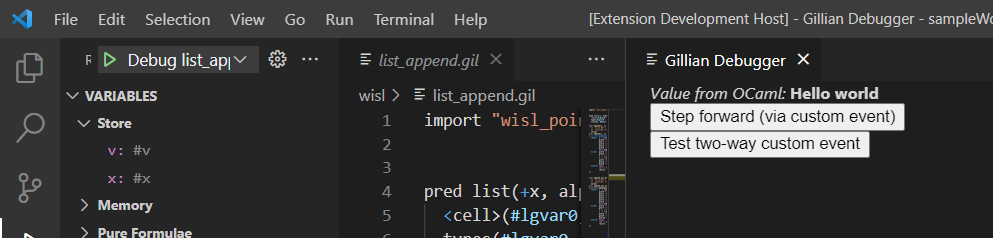
\includegraphics[width=400px]{img/webview-example.png}
  \caption{An example of a Webview created by a VSCode extension}
  \label{fig:webview-example}
\end{figure}




\myparagraph{Debug Adapter Protocol}
A common issue when adding IDE support for development tools is the sheer
number of editors that would ideally be supported~\cite{magpiebridge}. Whilst
VSCode has a huge market share, only supporting VSCode would neglect a
significant portion of developers. Unfortunately, maintaining support for many
editors at once is an unreasonably large undertaking. The \textit{Debug Adapter
Protocol} (DAP)~\cite{dap} exists as an attempted countermeasure to this issue,
turning the $O(m \times n)$ complexity problem of supporting many debuggers on
many editors into a $O(m + n)$ problem; each debugger and each editor need only
be integrated once.

\begin{figure}[!t]
  \centering
  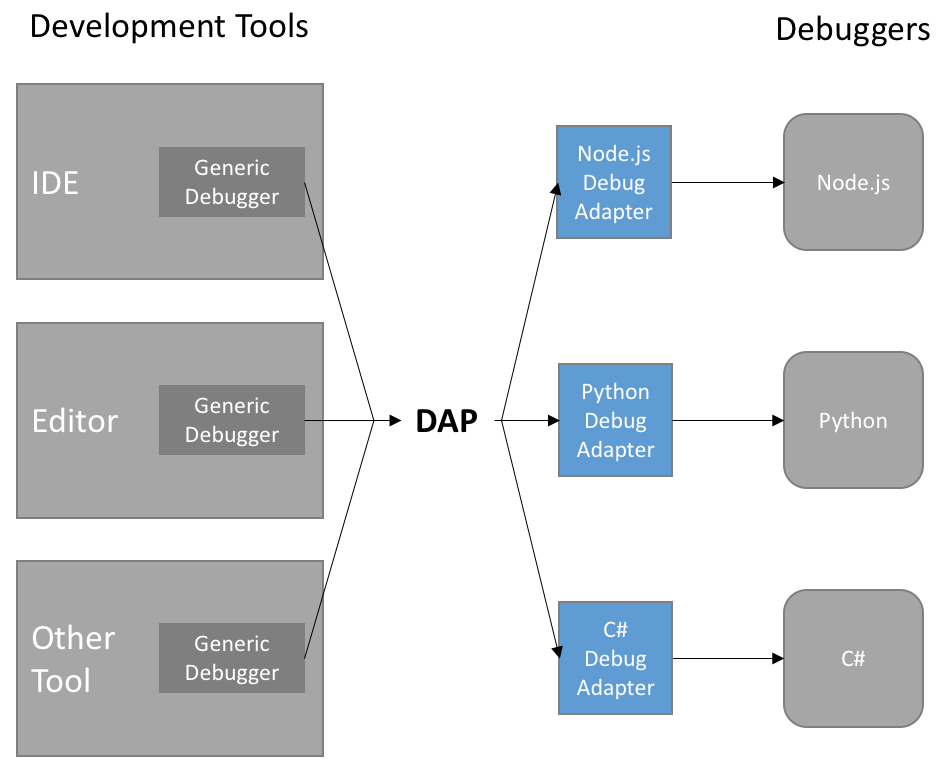
\includegraphics[width=0.5\textwidth]{img/dap-diagram.png}
  \caption{
    DAP: an interface between arbitrary IDEs and
    arbitrary debuggers~\cite{dap}.
  }
  \label{fig:dap-diagram}
\end{figure}

As discussed in \autoref{sec:intro}, the DAP's limited set of
included commands proved a limiting factor in the development of a Gillian
debugger. A potential solution is to make use of custom commands and events,
which is supported both by VSCode (sending custom requests
at~\cite{vscode-dap-custom-request}, receiving custom events
at~\cite{vscode-dap-custom-event} and the OCaml DAP
implementation currently used in Gillan's debugger~\cite{ocaml-dap} (where
custom events and commands are defined similarly to those already
provided~\cite{ocaml-dap-custom}).



\myparagraph{Inclusion of OCaml code}
Resulting of Ocsigen's work as part of their OCaml web framework
~\cite{ocsigen-framework}, OCaml programs can be directly compiled into
JavaScript using their \texttt{Js\_of\_ocaml} package~\cite{js-of-ocaml}; by
adding a compilation flag in a project's Dune file, the relevant program can be
compiled to a \texttt{.js} file instead of a native binary. This produced file
doesn't need to be used as its own program; using the provided JS
bindings~\cite{js-of-ocaml-bindings}, the resulting JS code can export
functions and values, just like normal JS code, to be used elsewhere in a
JavaScript project.

Another option is to make use of the OCaml VSCode bindings
~\cite{vscode-ocaml-bindings} provided by OCamlLabs'
\texttt{vscode-ocaml-platform}~\cite{vscode-ocaml-platform, ocamllabs}; this
way, no JavaScript need be written at all.

These options allow the line between JavaScript and OCaml to be drawn wherever
is most opportune; the extension could be written completely in JavaScript,
requiring more attention when interacting with Gillian's debugger; the
extension could be entirely OCaml, sacrificing more succinct integration with
VSCode for a more unified codebase with Gillian; it is just as possible to draw
the line somewhere in-between, exposing the more Gillian-related OCaml code via
functions to the JavaScript that communicates with VSCode. Additionally, both
scenarios allow for Gillian code to be shared with the extension. However,
with the Gillian libraries as they are, such libraries cannot be haphazardly
included in the extension code; \texttt{Js\_of\_ocaml} transitively includes all
OCaml dependencies, potentially leading to code that cannot be executed. As a
concrete example to this, attempting to include Gillian's \texttt{debugAdapter}
library results in erroring code, due to the compiler's attempt to include an
SQLite implementation, which it simply is not equipped to handle. Aside from
this, the inclusion of unnecessary dependencies in JS-compiled code results in
a hugely bloated extension - the \texttt{debugAdapter} example created a
compiled JS file over a million lines long. The ideal scenario here is to move
shared Gillian code to its own library within Gillian, which has as few
dependencies as possible (ideally none), but on which both Gillian and the extension
code would then depend.

\begin{sidewaysfigure}
  \center
  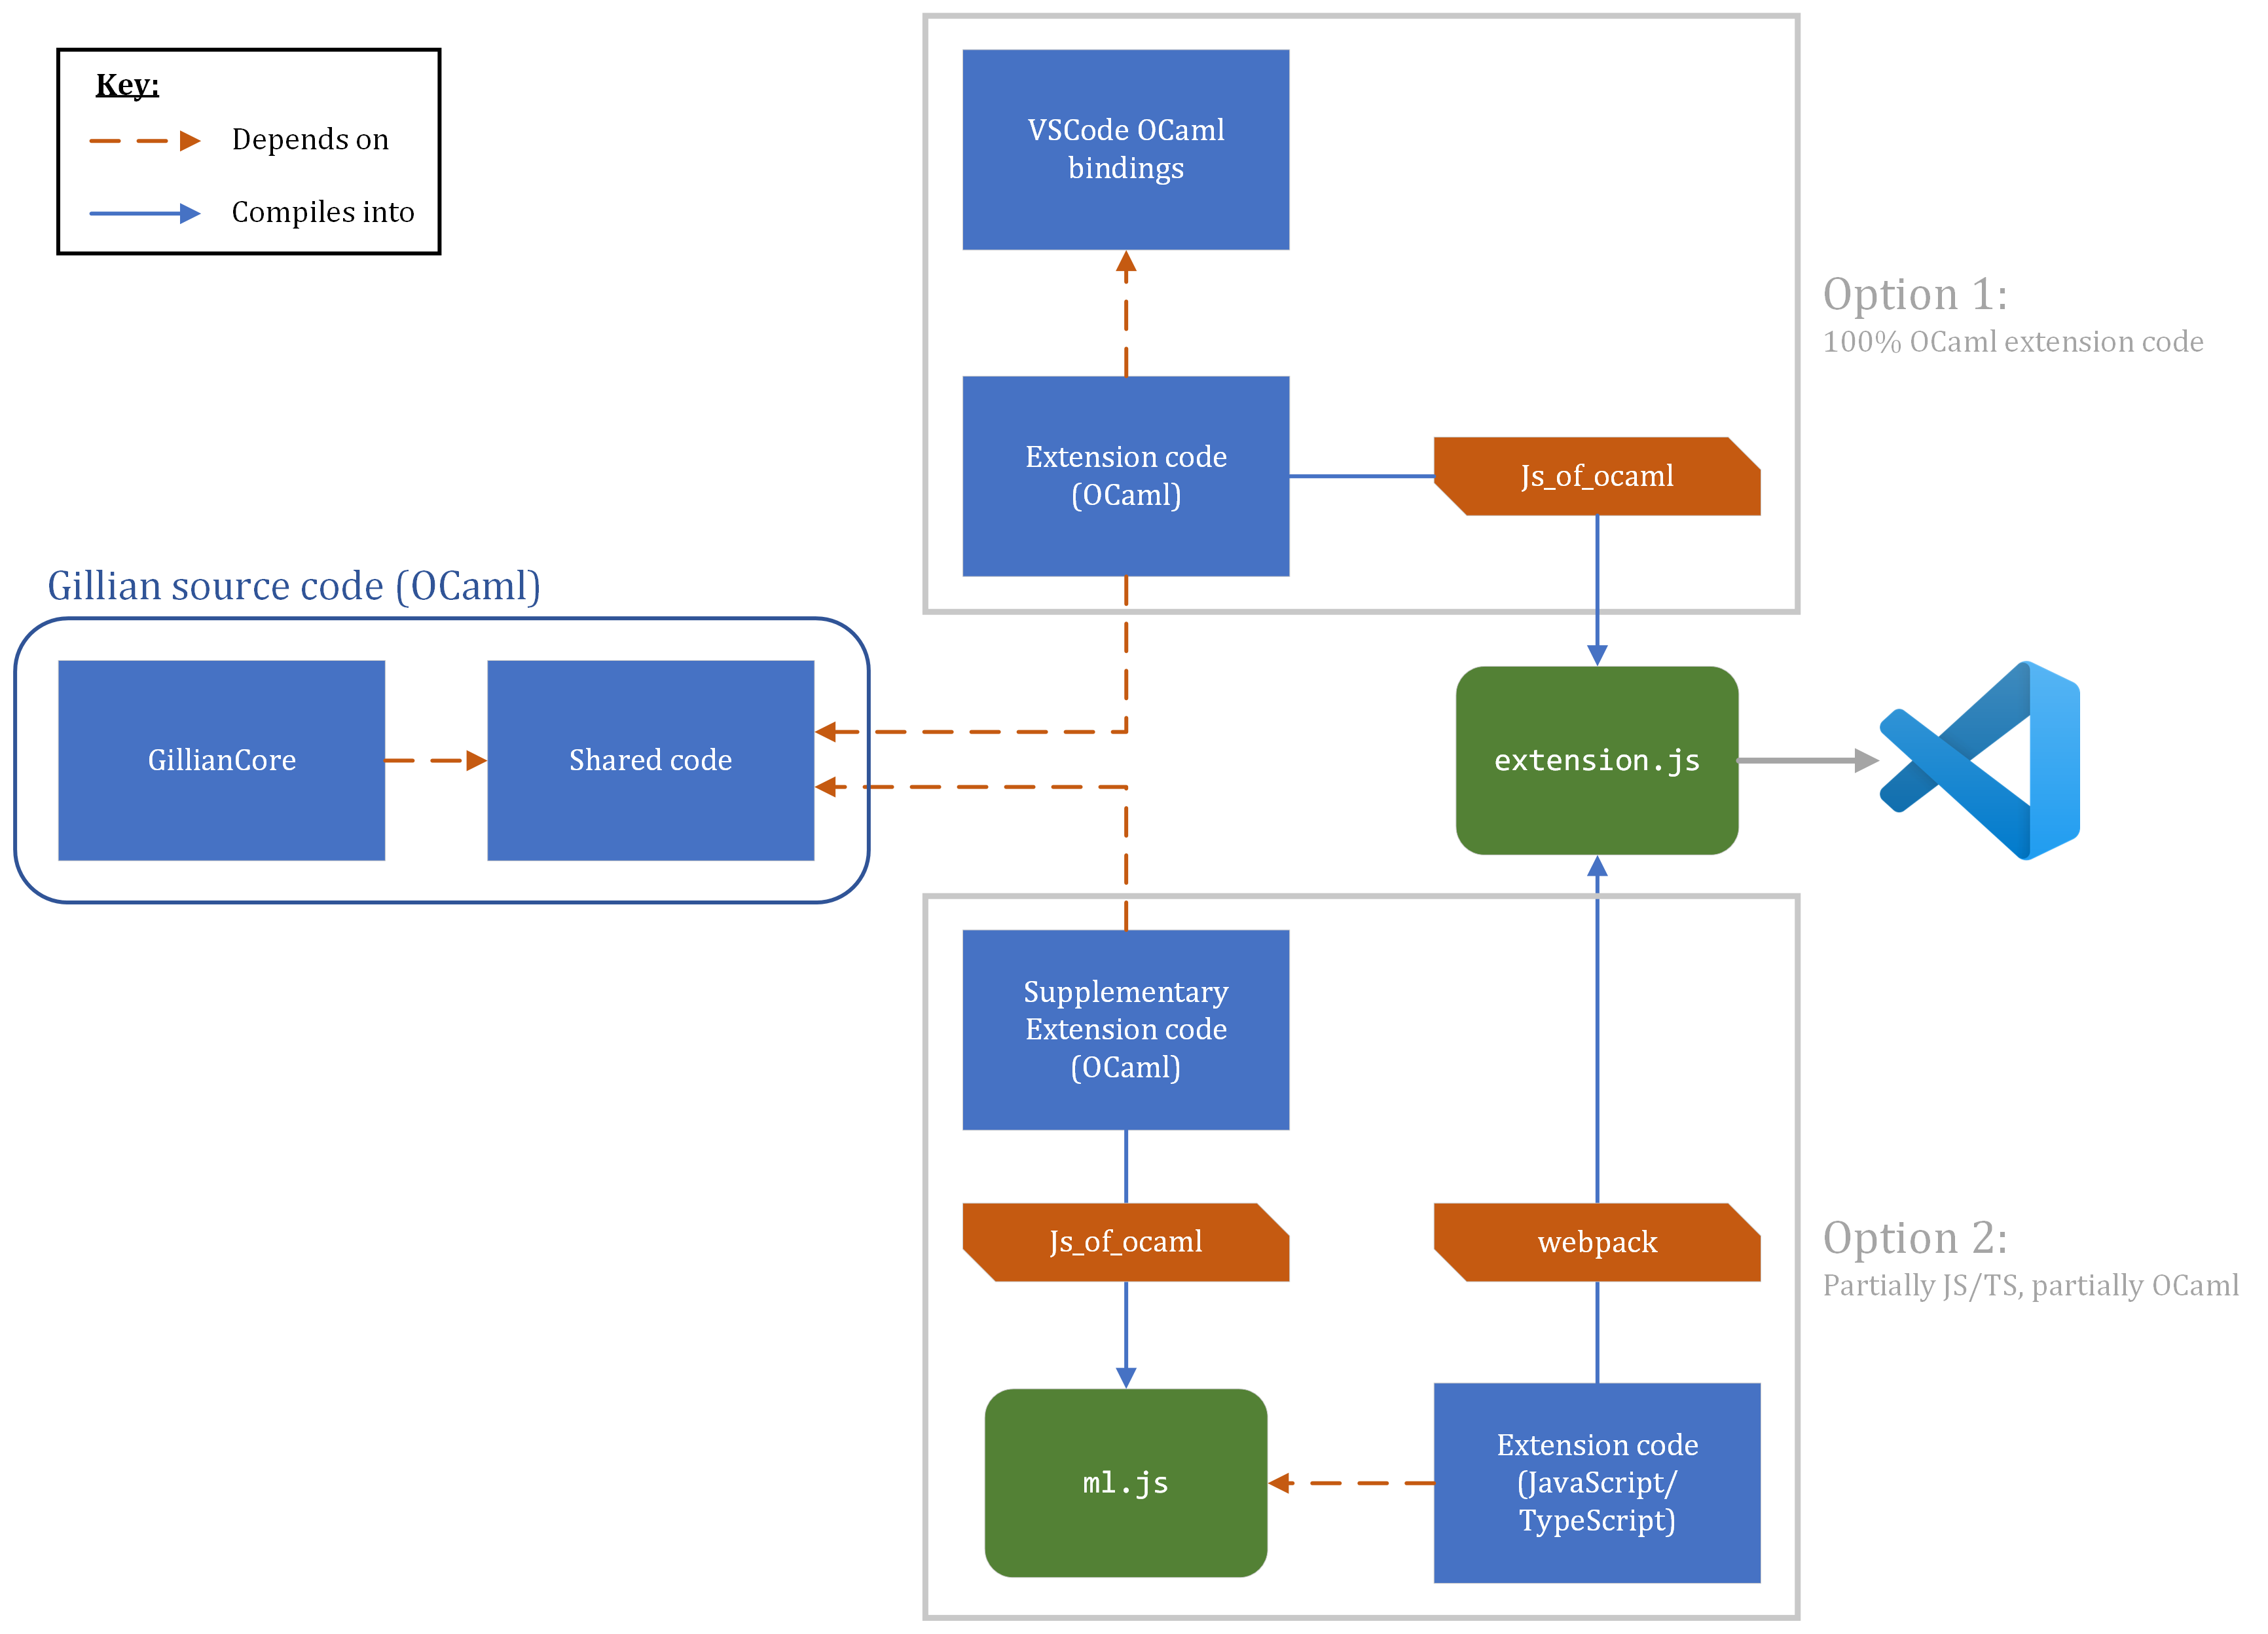
\includegraphics[width=0.8\textwidth]{img/vscode-extension-with-ocaml.png}
  \caption{The process of including OCaml code in a VSCode extension}
  \label{fig:vscode-extension-with-ocaml}
\end{sidewaysfigure}

\myparagraph{Putting it all together}
\label{sec:background:extending-dap}
A combination of DAP custom events and VSCode's Webviews could allow us to move
past DAP's initial limitations. This, however, comes at the cost of creating an
implementation specific to VSCode, eliminating a large benefit of using the DAP
in the first place.

A working example that tests custom DAP commands/events, Webviews and the
inclusion of OCaml code (alongside a Gillian library) is available at
\cite{debugger-experiment}.

\section{MagpieBridge}

Similarly to program debugging, adding support for static code analysers to IDEs
is limited by the amount of tools and IDEs that support must be added for. In a
similar notion to the DAP, MagpieBridge~\cite{magpiebridge} is `a framework for
integrating Static Analyses into IDEs and Editors with the Language Server
Protocol'~\cite{magpiebridge-repo}. The \textit{Language Server Protocol}
(LSP)~\cite{lsp} is another of Microsoft's creations, similar to the DAP, which
adds an arbitrary interface bridging IDEs and language tools (syntax checkers,
intellisense, etc.). As an example, MagpieBridge has provided fully
functional integration for~Infer~\cite{infer-ide}.

A particular feature of MagpieBridge is its ability to serve a configuration
webpage, in which the user can configure the static analysis in their browser
of choice. Unfortunately, this pre-generated page can't contain any custom
content, and can only be used for configuration - this would prohibit advanced
debugging features from being served directly from a MagpieBridge server.

Additionally, the inclusion of MagpieBridge would involve the addition of Java
to the language base of Gillian, increasing complexity of the project and
potentially harming long-term usability.


\begin{figure}
  \centering
  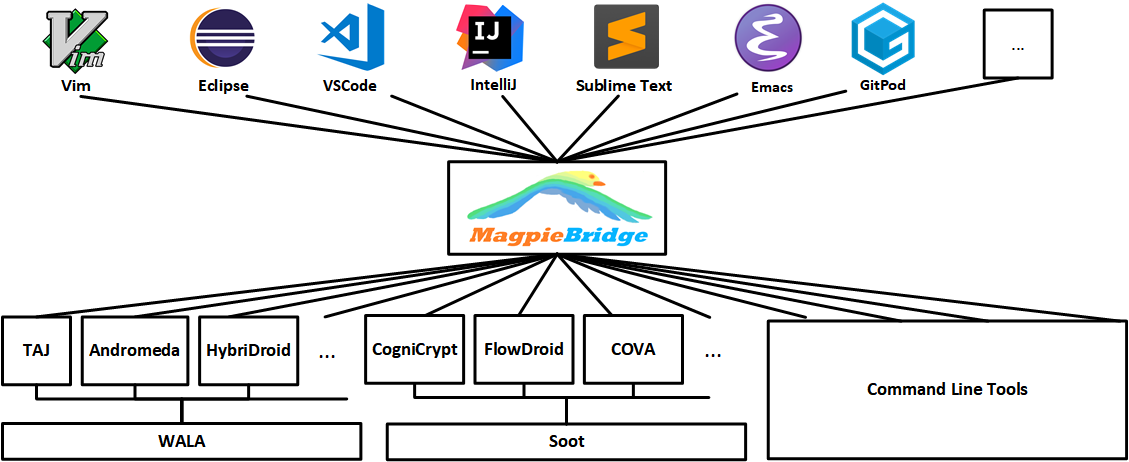
\includegraphics[width=\textwidth]{img/magpiebridge-goal.png}
  \caption{
    The goal of MagpieBridge; bridging static analysis tools with IDEs.
    From~\cite{magpiebridge-repo}.
  }
  \label{fig:magpiebridge-goal}
\end{figure}

%!TEX root = ../main.tex

\chapter{Project plan}\label{cha:plan}
\todo{Get rid of!}

The goals of the project, together with a rough timeline, are as follows:

\newcommand{\vertline}{\color{black}\makebox[0pt]{\textbullet}\hskip-0.5pt\vrule width 1pt\hspace{\labelsep}}

\begin{flushleft}
\begin{tabular}{@{\,}r <{\hskip 2pt}!{\vertline}>{\raggedright\arraybackslash}p{13cm}}

  December 2021 & Familiarise with previous project work           \newline
                  Begin preliminary research on VSCode and its API,
                  as well as the DAP                                 \newline \\
  January 2022  & $\longleftarrow$ \textit{Current time}             \newline
                  Read up on VSCode extensions, webviews, and
                  OCaml-to-JavaScript compilation            \newline
                  Complete an initial experiment with these
                  findings                                           \newline
                  Compile background research, complete interim report        \newline \\
  February & Deep dive into Gillian codebase, with focus on 
             debugging and unification                                                \newline \\
  March    & Implement stepping through unification plans          \newline \\
  April    & Implement custom debugging UI for VSCode, including
             branching execution and tree visualisation              \newline
             Add error lifting support for JavaScript debugging    \newline \\
  May      & Implement quality-of-life changes                     \newline
             Implement Rust debugging (if possible)                \newline \\
  June     & Finish implementation, finalise report                 
\end{tabular}
\end{flushleft}

Further, additional details concerning some parts of the plan are as follows:

\begin{itemize}
  \item The research concerning VSCode and its webviews and extensions, the
        DAP, and OCaml to JS compilation has already been completed; this
        serves the basis for \autoref{sec:background:engineering-tools}.

  \item \textbf{Unification}. A desired feature is the ability to step through
        Gillian's unification process, which stands as one of the pain points
        of the current user experience; a large share of verification errors
        occur when unifying against either the pre-condition of a called
        function, the post-condition of the current function, or the folding of a predicate. In the
        presence of several specifications, the process of identifying which
        specification or predicate definition \textit{should} be unifying (but isn't) often takes a
        significant amount of time and thought, when a bespoke interface would
        greatly streamline this process.

        In particular, unification is performed following tree-shaped
        \textit{unification plans}; the ability to step through and visualise
        progress in these plans would immediately give the developer a far
        better idea of the cause of a given unification error.

  \item The `quality-of-life' features penned in for later in the project
        represent small tweaks or features that the Gillian team (or any
        testers) think would be useful additions, provided there is ample time
        to implement them.

  \item Implementing a Rust debugger depends on the progress made in another
        final-year project running parallel to this one; its inclusion is not
        guaranteed, but it is also not necessary to the success of this project.

\end{itemize}

\section{Evaluation Plan} 

The measure of success for this project comes down to three factors:

\myparagraph{Evaluating against tools}
As it stands, VeriFast is Gillian's closest competitor; once the project is
completed, Gillian's debugger will be re-compared against VeriFast to see which
has the more usable debugging experience, and why. Another comparison worth
considering is Infer; given its widespread use in industry, the pursuit of
pushing Gillian's ease of use and clarity of error reporting to be comparible
to that of Facebook's tool is a worthy goal.

\myparagraph{Evaluating against examples}
This is a more personal form of evaluation; before embarking on this project,
the author of this project sat the course on Scalable Software Verification (a.k.a.~Separation Logic); common challenges set in this course were to create lemmas,
pre-/post-conditions, loop invariants, etc.\ that are appropriate for particular
programs, and to verify their correctness. A good measure of Gillian's progress
would be to attempt to use it to aid with solving such challenges. 
This part of the evaluation would ideally involve usability feedback from the members of the Verified Software group, as well as some of the students who sat the Separation Logic course.

\myparagraph{Pushing the debugger's limits}
The final frontier, as it were---upon completion of this project's
implementation, the debugger ought to be pushed to its limits, exploring the
`corners' of the debugger and what it can accomplish. This will be both a good
test of the debugger's capabilities, and a good indication of what future work
may be needed.


%!TEX root = ../main.tex
%chktex-file 17

\chapter{Evaluation}\label{sec:eval}

There is some difficulty in describing this project's merit, stemming somewhat
from its novelty, with it being the crescendo of several years of MEng/MSc
projects with the goal of making semi-automatic program verification accessible
to any who understand separation logic, not just the authors of Gillian. The
technical hurdles faced during the actual implementation were not particularly
profound (though are noteworthy nonetheless)\todo{What challenges?}, as the main challenge of this
project resided in both the broad and deep prerequisite understanding required
to marry the intricacies of Gillian with the practical aspects of the DAP,
VSCode's extension API, and modern web development---all within the limited time
span of an MEng final project. What should be noted is that there are few
competing projects in this space; those that do exist either have significantly
different goals (Infer), or exist only in a prototype stage (VeriFast). This
leads us to believe that this work could be potentially ground-breaking.

Due to the scarcity of similar tools, points of strong comparison for Gillian's
new debugger are few and far between. The best options to evaluate this project
against are the options available to Gillian users prior to this project (or
prior to any debugging work being done at all, as this project comes after
multiple years of work to this end), and to VeriFast, Gillian's closest
contemporary.

\section{Comparison with Previous Gillian Debugging Methods}

When compared to the previous debugging method---manually reading the (textual)
log file resulting from verification---the advantages of having a working visual
debugger are evident. Not only does the log file require a deep understanding of
Gillian's internals, but it contains a vast amount of detail, often obfuscating
the information relevant to the encountered error. Moreover, the navigation from
one point of interest to the next is highly non-trivial. Even in the simple case
of the recursive list length function, which was used as a baseline throughout
the project, a total of 9328 lines of logging output is generated during
verification. As a more precise comparison, about 1500 of those lines concern
unification of the postconditions, with a high degree of redundancy and
verbosity. This contrasts with what is essentially a few lines of text in the
debugger interface, with more detail available as and when the user requires.
Compared to the clear, clean, and concise interface of the new solution, a far
more ideal debugging process has been presented---even those with a deep
understanding of Gillian, who are well acclimated to debugging via the file log,
intend to use this as their primary method of debugging moving forwards.

\todo{Add a specific example --- reference background?}

The new debugger also brings substantial improvement when compared to the
previous iterations: aside from not having any unification information
whatsoever, their use required of the user to understand the quirks of the
solution, such as branches being executed one after the other with no means of
discerning between them. The iterations of the debugger were very much a case of
attempting to move Gillian a step closer to debugging in whatever manner was
available, rather than setting out a clear vision of what prospective users
would desire from a program verification debugger, and working to meet that
goal.

\section{Comparison with VeriFast}

VeriFast has a fundamentally different approach to the debugging process;
instead of reporting the results of symbolic execution step by step, the whole
verification is performed all at once, only showing details in the event of an
error (or a breakpoint being reached). There is no concept of exploring the
different execution paths of the program, severely limiting its ability to be
used as a tool for deepening one's understanding of the underlying reasoning.
Multiple branches of execution are not presented to the user, only showing the
single path taken to reach the error or breakpoint. This textual format is far
more rigid than the Gillian debugger's explorable execution map given in
\autoref{fig:verifast-path-compare}; not only is the latter more feature-rich,
but it also provides a complete overview of the program execution.

\begin{figure}
  \centering
  \begin{subfigure}[b]{0.4\textwidth}
    \center{}
    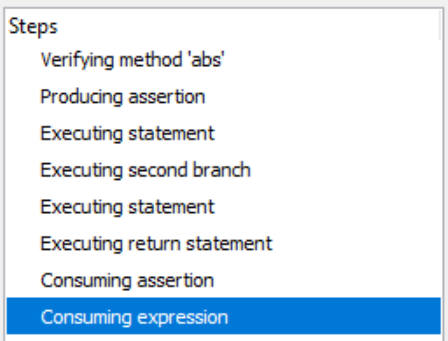
\includegraphics[width=0.75\textwidth]{img/verifast-path.png}
    %\caption{The execution path information given by VeriFast}%
    %\label{fig:verifast-path}
  \end{subfigure}
  \qquad
  \begin{subfigure}[b]{0.4\textwidth}
    \centering
    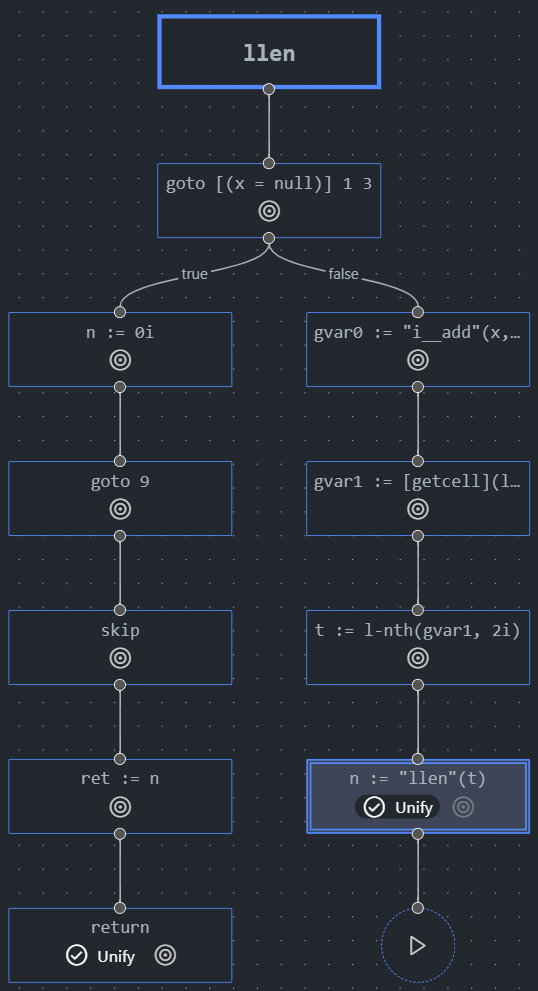
\includegraphics[width=0.9\textwidth]{img/execmap-final.png}
    %\caption{The Gillian debugger's execution map}%
    %\label{fig:execmap-final}
  \end{subfigure}
  \caption{Execution Path/Branching Information: \textbf{(a)} VeriFast (left); 
  \textbf{(b)} the Gillian debugger (right)}%
  \label{fig:verifast-path-compare}
\end{figure}

VeriFast also gives no insight into the unification process; the only
information provided is an error message should unification fail. The Gillian
debugger gives more information to this end by showing all assertions from
a unification, up to and including the failing one, as shown in
\autoref{fig:verifast-path-compare}.

\begin{figure}
  \centering
  \begin{subfigure}[b]{0.4\textwidth}
    \center{}
    
\includegraphics[width=0.9\textwidth]{img/verifast-error.png}
    %\caption{A unification error given by VeriFast}%
    %\label{fig:verifast-error}
  \end{subfigure}
  \qquad
  \begin{subfigure}[b]{0.4\textwidth}
    \centering
    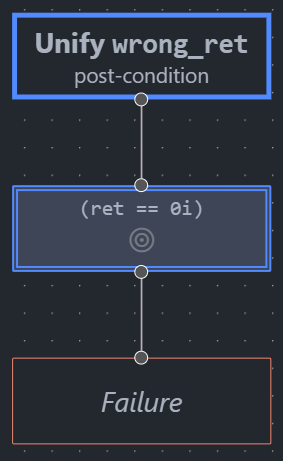
\includegraphics[width=0.3\textwidth]{img/unifymap-failure.png}
    %\caption{A failing unification map given by the Gillian debugger}%
    %\label{fig:unifymap-failure}
  \end{subfigure}
  \caption{Failing Unification Information: \textbf{(a)} VeriFast (left);
  \textbf{(b)} Gillian debugger (right)}%
  \label{fig:verifast-unifyfail-compare}
\end{figure}

Another point of comparison is the accessibility of the different solutions.
VeriFast is a completely isolated tool, its graphical interface needing to be
run separately from any other software used for development. Now, armed with the
new debugging functionality, developers have a real possibility of using Gillian
as part of their development pipeline; the ability to debug Gillian verification
directly inside VSCode (by far the most popular editor in the world) is, we
believe, a previously unmatched level of accessibility for a tool of this
purpose.


\section{Limitations}%
\label{sec:eval:limitations}

Although this project has made substantial progress towards making Gillian a
more user-friendly and mainstream tool, there are still several limitations that
need to be addressed.

\myparagraph{Incomplete target language lifting.}
As discovered in \autoref{sec:debug-interface}, the mechanism to lift the
debugging process to the level of the target language is currently incomplete,
due to particular mechanisms of how multiple GIL commands are coalesced back
into a single target language command, preventing full support for lifting
execution maps to represent the target language.
Thankfully, these issues are very low-hanging fruit. However, the challenges
involved in supporting lifting for more of the verification process could
constitute another entire Masters project on their own, such as lifting the
symbolic state, and various kinds of errors, to a point where no knowledge of
GIL would be required to debug the verification of a program written in a
supported target language (for example, JavaScript).

\myparagraph{Lack of annotations on the GIL AST.}
The current debugger highlights which part of the code is being symbolically
executed; however, there is no such mechanism during unification.
For example, the debugger does not highlight what part of the state is being
affected by a particular assertion. The addition of state highlighting, or even
highlighting previous parts of code that were the last to affect parts of the
state, would do much to create a more intuitive connection between the code and
the unification process.

\myparagraph{Performance.}
Logging in Gillian is quite slow. In the past, the creators of Gillian put much
effort into minimising the overhead of the logging infrastructure when logging
is disabled. Executing verification and logging into a file (the old way) is
about 5.75\footnotemark[1]{} times slower than executing verification with
logging disabled. In the new infrastructure, executing verification and logging
to the database is 2.32\footnotemark[1]{} times slower than when logging into
the file, thus 13.35\footnotemark[1]{} times slower than no logging at all.
For small WISL programs, such as those studied in the Separation Logic course,
programs are simple enough for this time difference to be negligible. However,
full verification of the fragment of the \texttt{AWS Encryption SDK} takes about
6 minutes on a modern high-end laptop, meaning the relative performance of the
debugger would be far too sluggish for mainstream use. \footnotetext[1]{Measures
performed on the available benchmark for WISL verification.} That being said,
our expertise gives us confidence that these performance numbers can be
greatly improved upon with a relatively small amount of work.
The two most obvious improvements are \textbf{(1)} making the database
interaction asynchronous (or potentially multithreaded), and \textbf{(2)}
finding a more efficient method of serialising data than JSON---perhaps
Protocol Buffers~\cite{protobuf}. Interestingly, implementing \textbf{(1)} may
result in database logging becoming more efficient than logging into a file,
since file-logging must be performed synchronously as to preserve the order of
the logs, while records can be written in any order in the database while
preserving the necessary structure.

\myparagraph{Tool-developer experience.}
However powerful the logging structure is, its API is far from perfect at
present. Retrieving previously logged data from the database requires writing
SQL queries by hand, followed by calling the OCaml-SQL driver. However, given
the principled structure of the log trace, this experience could be largely
improved by designing a domain-specific query language adapted to extracting any
kind of information from the traces. Note, however, that this limitation only
affects the tool developer, and does not affect the primary customer of this
project, the tool user.

Of course, none of these factors detract from the fact that, from the
perspective of user experience, this project has elevated Gillian from a
prototype research tool to one that that proves useful in pursuing new research
in program analysis, and even more importantly, a tool that can be used for
educational purposes---to help those having their first experience of
program analysis, separation logic, and symbolic execution form a deeper
understanding by automatically applying its principles to actual programs.


\section{Reflection}

As to be expected, this project was a significant learning experience, both
reinforcing good practices and showing areas for improvement. Outlined here are
some reflections of note thinking back over the project.

\myparagraph{Planning and logistics.}
Despite development on the project finishing up closer to the deadline than
would be desired, we believe that on the whole, the available time was used
wisely. The larger-than-expected amount of time spent on development was a
result of the project's ambition rather than poor planning; in fact, strong
plans made at various points through the project ensured that development could
be halted when necessary to leave the remaining unimplemented features for
future work, while still providing enough of a substantial improvement to form
a fully realised submission and meet the project's main goals---for example,
while basic support for debugging unification was deemed core to the project,
it was deemed acceptable to leave the tree-based interface for unification
unfinished, should it be necessary to meet the project deadline.

\myparagraph{Personal thoughts.}
Personally speaking, the project reinforced the importance of frequent and clear
communication with supervisors. Sacha and Petar were endlessly helpful and
practically always available, though I feel as though I may not have used such
an enviable position to its fullest advantage; while I think I did a relatively
good job of keeping my supervisors updated as to demonstrate consistent progress
being made, I should have more frequently described specifically what I was
working on and the motivations behind it, as this project was not entirely
without time wasted, due to a lack of direction leading to a tangent of
unnecessary development or research. Despite that, it's important to note that
there were no costly roadblocks during the project, so smaller optimisations
like the aforementioned are the next best thing to consider improving.

\myparagraph{In hindsight.}
If this project were repeated with the gift of foresight, research into the
inner workings on Gillian earlier should be performed earlier into the project;
it was not entirely apparent ahead of time how much of the project's difficulty
came from the various areas of required understanding (as outlined at the start
of this section) required to begin substantial development work.

%!TEX root = ../main.tex

\chapter{Ethical Discussion}\label{sec:ethics}
\todo{This is copied from interim; does it need changing?}

As Gillian's nature is to verify a program's correctness, a natural consequence of Gillian is the discovery of bugs in applications, particularly memory-related bugs.
This was evident when Gillian was used to verify parts of AWS's encryption SDK in both C and JavaScript, which led to the discovery of 5 total bugs, two of which were security vulnerabilities (one in C, one in JS)~\cite{gillian-part2}.
This is often the case with memory-related bugs; Microsoft has reported that across their products, over the course of 2006 to 2018, consistently around 70\% of addressed security vulnerabilities concerned memory safety~\cite{microsoft-memory-bugs}.
Thus, there exists the possibility of malicious parties using Gillian to uncover security vulnerabilities by finding bugs in an organisation's code and its management of memory.

However, such an eventuality would be highly unlikely, as the malicious party would have to:
\begin{itemize}
  \item Have a working understanding of separation logic
  \item Deduce the intentions of the victim's code to the extent that they can write valid and relevant assertions for said code
  \item Be lucky enough to analyse a section of code that actually contains a vulnerability
\end{itemize}

In such a constellation of events, the completion of this project might aid the attacker in understanding the nature of the discovered vulnerability.

Because of these factors, it is clear that the benefits of Gillian and the improvement of its debugging capabilities far outweigh the slight possibility in it aiding cyberattacks.
The chance of a malicious party being aided in their attacks by Gillian is negligible compared to the possibility of the potential victim using Gillian to discover and subsequently fix vulnerabilities before they are discovered.
\chapter{References}\label{cha:refs}

\makeatletter
\let\oldchapter=\chapter{}
\renewcommand{\chapter}{\@gobbletwo}
\makeatother
\bibliographystyle{acm}
\bibliography{refs}
\let\chapter=\oldchapter{}


\end{document}
